\documentclass[border=0pt]{standalone}
\usepackage{xcolor}
\usepackage{tikz,tikz-3dplot}
\begin{document}
	\tdplotsetmaincoords{50}{130}
    \begin{tikzpicture}
    % ---------------------------------------------------------
    \node at (5.2, 3.75) {{\bf Step 1: Shape Prior}};
    
    \node[rectangle,draw=black,anchor=west] (prior) at (-1,2.5) {
        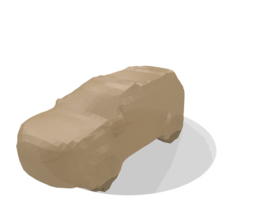
\includegraphics[height=1cm,trim={1cm 1.5cm 3.5cm 3cm},clip]{../gfx/overview_large/00010_target_off}
        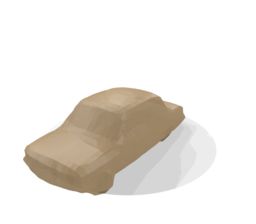
\includegraphics[height=1cm,trim={1cm 1.5cm 3.5cm 3cm},clip]{../gfx/overview_large/00004_target_off}
        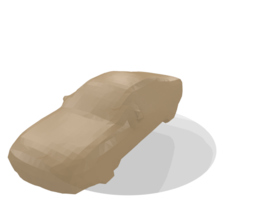
\includegraphics[height=1cm,trim={1cm 1.5cm 3.5cm 3cm},clip]{../gfx/overview_large/00000_target_off}
        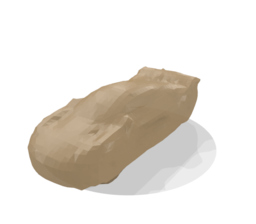
\includegraphics[height=1cm,trim={1cm 1.5cm 3.5cm 3cm},clip]{../gfx/overview_large/00012_target_off}
    };
    \node at (1.6,3.3) {\footnotesize Synthetic Training Data, e.g., ShapeNet};
    
    \node[] (y) at (0, -1.5) {\footnotesize Shape $y$};
    
    \node[rectangle,draw=black,anchor=west] (input) at (-1, 0) {
        \begin{tabular}{c}
            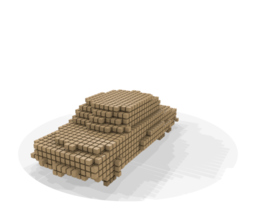
\includegraphics[height=1cm,trim={1cm 1.5cm 3.5cm 3cm},clip]{../gfx/overview_large/00004_target_binvox}\\
            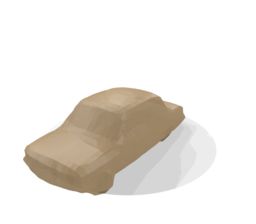
\includegraphics[height=1cm,trim={1cm 1.5cm 3.5cm 3cm},clip]{../gfx/overview_large/00004_target_off}
        \end{tabular}
    };  
    \node at ($(input.north) + (0,0.2)$) {\scriptsize $24{\times}54{\times}24$};
    
    \draw[-] ($(input.north east) + (0.2,0)$) rectangle ($(input.south east) + (0.55,0)$);
    \node[rotate=90] at ($(input.east) + (0.375,0)$) {\scriptsize conv+pool};
    \node[anchor=south west] at ($(input.north east) + (0.2,0)$) {\scriptsize $12{\times}18{\times}12$};
    \draw[-] ($(input.north east) + (0.7,-0.25)$) rectangle ($(input.south east) + (1.05,0.25)$);
    \node[rotate=90] at ($(input.east) + (0.875,0)$) {\scriptsize conv+pool};
    \node[anchor=south west] at ($(input.north east) + (0.7,-0.25)$) {\scriptsize $6{\times}6{\times}6$};
    \draw[-] ($(input.north east) + (1.2,-0.5)$) rectangle ($(input.south east) + (1.55,0.5)$);
    \node[rotate=90] at ($(input.east) + (1.375,0)$) {\scriptsize conv+pool};
    \node[anchor=south west] at ($(input.north east) + (1.2,-0.5)$) {\scriptsize $2{\times}2{\times}2$};
    
    \node (z) at (2.75, 0) {\footnotesize $z$};
    
    \node[rectangle,draw=black,anchor=east] (output) at (6.5, 0) {
        \begin{tabular}{c}
        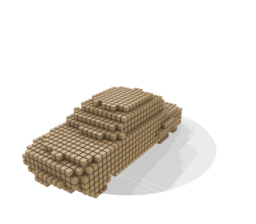
\includegraphics[height=1cm,trim={1cm 1.5cm 3.5cm 3cm},clip]{../gfx/overview_large/00004_prediction_binvox}\\
        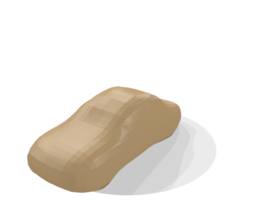
\includegraphics[height=1cm,trim={1cm 1.5cm 3.5cm 3cm},clip]{../gfx/overview_large/00004_prediction_off}
        \end{tabular}
    };
    
    \draw[-] ($(output.north west) - (0.2,0)$) rectangle ($(output.south west) - (0.55,0)$);
    \node[rotate=90] at ($(output.west) - (0.375,0)$) {\scriptsize conv+nnup};
    \draw[-] ($(output.north west) - (0.7,0.25)$) rectangle ($(output.south west) - (1.05,-0.25)$);
    \node[rotate=90] at ($(output.west) - (0.875,0)$) {\scriptsize conv+nnup};
    \draw[-] ($(output.north west) - (1.2,0.5)$) rectangle ($(output.south west) - (1.55,-0.5)$);
    \node[rotate=90] at ($(output.west) - (1.375,0)$) {\scriptsize conv+nnup};
    
    \node (ry) at (5.5, -1.5) {\footnotesize Rec. Shape $\tilde{y}$};
    
    \node[] (L) at (2.75, -1.9) {\footnotesize Reconstruction Loss};
    
    \draw[-] (ry) -- ($(ry) - (0,0.4)$);
    \draw[-] ($(ry) - (0,0.4)$) -- (L);
    \draw[-] (y) -- ($(y) - (0,0.4)$);
    \draw[-] ($(y) - (0,0.4)$) -- (L);
    
    % --
    \draw[-] (3.5, 1.25) -- (3.5, 1.5);
    \draw[-] (3.5, 1.5) -- (12.5, 1.5);
    \draw[->] (12.5, 1.5) -- (12.5, 1.25);
    \node at (7.25, 1.75) {\footnotesize retain fixed decoder};
    \draw[-,dashed] (7.25,-2.15) -- (7.25,1.45);
    \draw[-,dashed] (7.25,2) -- (7.25,2.45);
    \draw[-,dashed] (7.25,3) -- (7.25,4.05);
    
    \node at (7.25, 2.75) {\footnotesize\textbf{no correspondence needed}};
    \begin{scope}[shift={(9,0)}]
    
    % ---------------------------------------------------------
    \node at (0.7, 3.75) {{\bf Step 2: Shape Inference}};
    
    \node[rectangle,draw=black,anchor=east] (inference) at (6.5,2.5) {
        
\includegraphics[height=1cm,trim={1cm 1.5cm 3.5cm 3cm},clip]{../gfx/overview_large/00037_input_txt}
        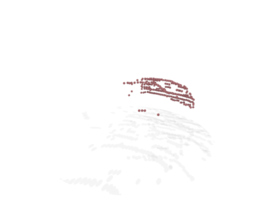
\includegraphics[height=1cm,trim={1cm 1.5cm 3.5cm 3cm},clip]{../gfx/overview_large/00005_input_txt}
        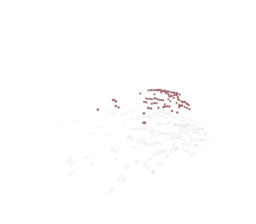
\includegraphics[height=1cm,trim={1cm 1.5cm 3.5cm 3cm},clip]{../gfx/overview_large/00045_input_txt}
        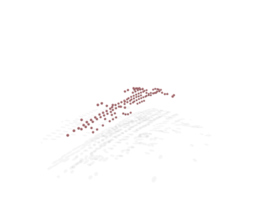
\includegraphics[height=1cm,trim={1cm 1.5cm 3.5cm 3cm},clip]{../gfx/overview_large/00047_input_txt}
    };
    \node at (3.8,3.3) {\footnotesize Real Training Data w/o Targets, e.g., KITTI};
    
    % --
    \draw[-,dotted] (prior) -- (inference);
    
    \node[] (y) at (0, -1.5) {\footnotesize Observation $x$};
    
    \node[rectangle,draw=black,anchor=west] (input) at (-1, 0) {
        \begin{tabular}{c}
        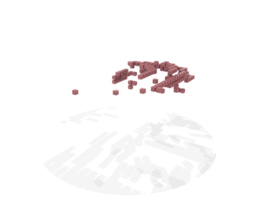
\includegraphics[height=1cm,trim={1cm 1.5cm 3.5cm 3cm},clip]{../gfx/overview_large/00037_input_binvox}\\
        
\includegraphics[height=1cm,trim={1cm 1.5cm 3.5cm 3cm},clip]{../gfx/overview_large/00037_input_txt}
        \end{tabular}
    };
    
    \draw[-] ($(input.north east) + (0.2,0)$) rectangle ($(input.south east) + (0.55,0)$);
    \node[rotate=90] at ($(input.east) + (0.375,0)$) {\scriptsize conv+pool};
    \draw[-] ($(input.north east) + (0.7,-0.25)$) rectangle ($(input.south east) + (1.05,0.25)$);
    \node[rotate=90] at ($(input.east) + (0.875,0)$) {\scriptsize conv+pool};
    \draw[-] ($(input.north east) + (1.2,-0.5)$) rectangle ($(input.south east) + (1.55,0.5)$);
    \node[rotate=90] at ($(input.east) + (1.375,0)$) {\scriptsize conv+pool};
    
    \node (z) at (2.75, 0) {\footnotesize $z$};
    
    \node[rectangle,draw=black,anchor=east] (output) at (6.5, 0) {
        \begin{tabular}{c}
        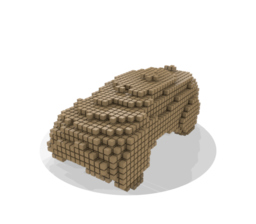
\includegraphics[height=1cm,trim={1cm 1.5cm 3.5cm 3cm},clip]{../gfx/overview_large/00037_prediction_binvox}\\
        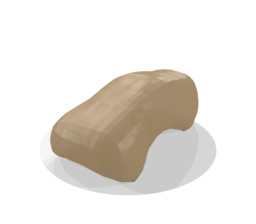
\includegraphics[height=1cm,trim={1cm 1.5cm 3.5cm 3cm},clip]{../gfx/overview_large/00037_prediction_off}
        \end{tabular}
    };
    
    \draw[-] ($(output.north west) - (0.2,0)$) rectangle ($(output.south west) - (0.55,0)$);
    \node[rotate=90] at ($(output.west) - (0.375,0)$) {\scriptsize conv+nnup};
    \draw[-] ($(output.north west) - (0.7,0.25)$) rectangle ($(output.south west) - (1.05,-0.25)$);
    \node[rotate=90] at ($(output.west) - (0.875,0)$) {\scriptsize conv+nnup};
    \draw[-] ($(output.north west) - (1.2,0.5)$) rectangle ($(output.south west) - (1.55,-0.5)$);
    \node[rotate=90] at ($(output.west) - (1.375,0)$) {\scriptsize conv+nnup};
    
    \node (ry) at (5.5, -1.5) {\footnotesize Prop. Shape $\tilde{y}$};
    
    \node[] (L) at (2.75, -1.9) {\footnotesize Maximum Likelihood Loss};
    
    \draw[-] (ry) -- ($(ry) - (0,0.4)$);
    \draw[-] ($(ry) - (0,0.4)$) -- (L);
    \draw[-] (y) -- ($(y) - (0,0.4)$);
    \draw[-] ($(y) - (0,0.4)$) -- (L);
    \end{scope}
    \end{tikzpicture}
\end{document}
